\newpage
% ==========================================
%               CHAPTER TWO
% ==========================================
\thispagestyle{plain}

\begin{center}
    \vspace*{0.5cm}
    {\large \textit{Chapter Two}} \\[0.4cm]
    {\Large \textbf{2 \quad LITERATURE REVIEW}}
\end{center}
\addcontentsline{toc}{chapter}{\textbf{2 \quad LITERATURE REVIEW}}
\vspace{0.45in}

\normalsize
\startchapterfloats{2}

\noindent Chapter~1 stated the problem, objectives, and scope of Eshara: a \textbf{web-only}, webcam-driven bilingual sign-language system with four standalone recognition models. This chapter reviews the literature that motivates those design choices. The review proceeds in a deliberate funnel: technological history of SLR (Section~2.1); machine-learning foundations (Section~2.2); computer-vision input representations (Section~2.3); deep-learning architectures (Section~2.4); pose-estimation frameworks (Section~2.5); datasets (Section~2.6); bilingual and Arabic research (Section~2.7); real-time web deployment (Section~2.8); the research gap Eshara addresses (Section~2.9); and a consolidated comparison of the four graduation models (Section~2.10). Chapters~3 and~4 implement the protocols justified here; Chapter~6 reports offline accuracy and Chapter~5 reports live web performance.\par\vspace{0.3cm}

% --- 2.1 HISTORY ---
\noindent\textbf{2.1\quad HISTORY OF SIGN-LANGUAGE RECOGNITION}\par
\addcontentsline{toc}{section}{\numberline{2.1}HISTORY OF SIGN-LANGUAGE RECOGNITION}
\vspace{0.2cm}

\noindent Three terms recur throughout this thesis and the SLR literature. \textbf{Sign-language recognition (SLR)} maps signing video or pose features to discrete \textbf{gloss} labels (individual signs). \textbf{Sign-language translation (SLT)} maps entire signing utterances to spoken-language sentences, often without an explicit gloss intermediate~\cite{camgoz2018neural}. \textbf{Isolated} SLR classifies one sign per clip; \textbf{continuous} SLR or CSLR decodes unsegmented video into gloss sequences~\cite{koller2020weakly,duarte2021how2sign}. Eshara implements isolated SLR only: the user deliberately signs one letter or one word at a time. Continuous translation is acknowledged as future work in Chapter~9.\par\vspace{0.2cm}

\noindent Sign-language recognition (SLR) has evolved through three broad technological phases, each driven by hardware availability and the maturation of machine-learning methods~\cite{rastgoo2021survey,sterpu2018sign,adaloglou2022comprehensive}. In the 1990s and early 2000s, researchers relied on instrumented gloves, accelerometers, and magnetic trackers that measured joint angles directly. Starner et al.\ demonstrated real-time American Sign Language recognition from wearable and desk-mounted cameras paired with specialised sensing equipment~\cite{starner1998realtime}. These approaches achieved usable accuracy in controlled settings but required expensive hardware and were unsuitable for everyday communication by deaf and hard-of-hearing users, who number in the hundreds of millions worldwide~\cite{who2024hearing}. The fundamental lesson from this era is that high-quality sensing does not guarantee deployability: assistive tools must work with hardware users already own.\par\vspace{0.2cm}

\noindent From the mid-2000s onward, commodity RGB cameras enabled vision-based systems that tracked hand shape and motion without worn sensors. Hidden Markov Models (HMMs) treated signing as a sequence of discrete visual states and remained the dominant statistical framework for more than a decade~\cite{rabiner1989tutorial,koller2015continuous,koller2016continuous}. HMMs are effective when hand segmentation is reliable and vocabularies are small, but they struggle with high intra-class variation in unconstrained webcam video. The introduction of depth cameras such as Microsoft Kinect around 2010 enabled skeleton joints to be recovered without gloves; however, depth hardware never achieved universal adoption in laptops and phones, limiting long-term impact for consumer-facing assistive products~\cite{rastgoo2021survey}.\par\vspace{0.2cm}

\noindent Convolutional neural networks (CNNs) later replaced hand-crafted features for many SLR pipelines, learning spatial filters directly from pixels or optical-flow stacks~\cite{he2016deep,koller2016continuous,pigou2018sign}. CNN-based isolated sign classifiers routinely exceed 90\,\% accuracy on curated benchmarks, yet still exhibit sensitivity to background clutter, lighting variation, signer skin tone, and camera resolution. Koller et al.\ advanced \emph{continuous} sign recognition through hybrid CNN--HMM architectures trained on broadcast footage, establishing a research line that later extended to weakly supervised sequence learning when frame-level gloss labels are incomplete~\cite{koller2020weakly}. This distinction between \emph{isolated} sign classification (one sign per clip) and \emph{continuous} recognition (unsegmented sentences) is central to Eshara: the graduation system solves isolated letter and word recognition; sentence-level gloss alignment is deferred to future work~\cite{duarte2021how2sign,forster2014rwth}.\par\vspace{0.2cm}

\noindent A third phase began with robust single-camera pose estimation. OpenPose demonstrated that body keypoints could be recovered in real time from monocular video~\cite{cao2019openpose}, and Google's MediaPipe extended this to efficient hand and body landmark extraction on consumer hardware~\cite{zhang2020mediapipe,bazarevsky2020blazepose}. Recent sign-language systems increasingly operate on skeleton or landmark feature vectors rather than raw pixels, reducing data requirements and enabling browser-side extraction~\cite{adaloglou2022comprehensive}. Parallel research on continuous sign-language recognition and sign-language translation treats entire sentences as sequences of glosses, typically using hybrid convolutional-recurrent or transformer encoders~\cite{camgoz2018neural,duarte2021how2sign}. The present project, Eshara, sits in a \textbf{hybrid isolated-sign paradigm}: letters and ArSL words use MediaPipe landmarks; ASL words use buffered RGB clips. The system recognises individual letters and short isolated word signs from a standard webcam, and leaves full continuous translation to Chapter~9.\par\vspace{0.2cm}

\begin{figure}[H]
\centering
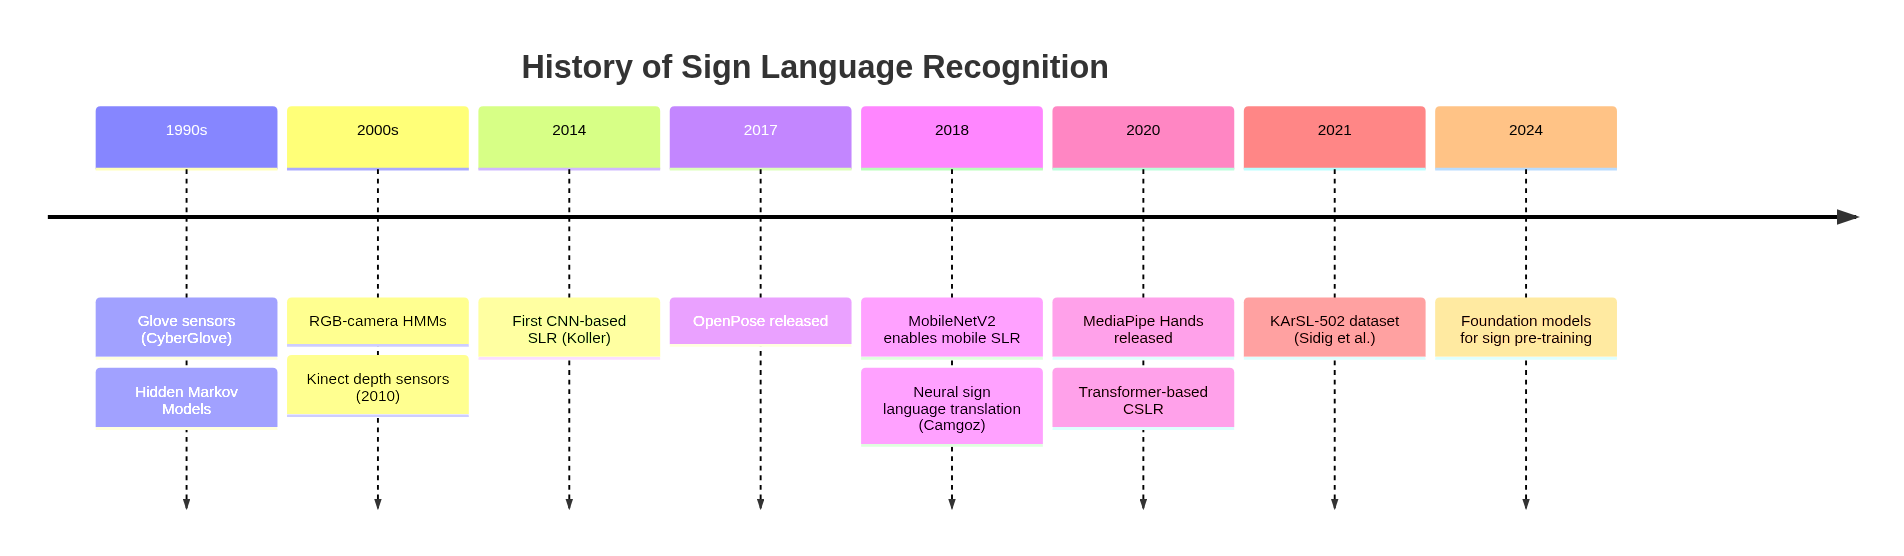
\includegraphics[width=0.92\textwidth]{images/fig_2-1_slr_timeline.png}
\caption{Evolution of sign-language recognition from sensor gloves and HMM-based RGB pipelines to landmark-based deep learning on commodity webcams.}
\label{fig:slr-timeline}
\end{figure}
\vspace{0.2cm}

\noindent As summarised in Figure~\ref{fig:slr-timeline}, the timeline captures the milestones above. The following table interprets the timeline in terms of \emph{what the system measures}, \emph{what model family dominated}, and \emph{whether ordinary users could deploy it} --- three questions that directly motivated Eshara's design.\par\vspace{0.2cm}

\begin{table}[H]
\centering
\caption{Interpretation of SLR technological eras (aligned with Figure~\ref{fig:slr-timeline}).}
\label{tab:slr-eras}
\small
\begin{tabular}{|P{1.35cm}|P{2.55cm}|P{2.35cm}|P{1.75cm}|P{2.9cm}|}
\hline
\multicolumn{1}{|c|}{\textbf{Period}} & \multicolumn{1}{|c|}{\textbf{Input to classifier}} & \multicolumn{1}{|c|}{\textbf{Dominant models}} & \multicolumn{1}{|c|}{\textbf{Deployability}} & \multicolumn{1}{|c|}{\textbf{Relevance to Eshara}}\\
\hline
1990s & Glove joint angles & HMM, template matching & Low (wearable hardware) & Historical only \\
\hline
2000s--2010 & RGB pixels, depth maps & HMM, early CNN & Medium (lab cameras) & Motivated vision path \\
\hline
2014--2017 & CNN features from video & CNN, CNN+HMM & Medium--high & Informed CNN trials \\
\hline
2017--2020 & Body/hand keypoints & CNN+RNN, attention & Rising & OpenPose/MediaPipe era \\
\hline
2020--2024 & Landmark vectors & BiLSTM, Transformer & \textbf{High} (webcam + browser) & \textbf{Eshara's era} \\
\hline
\end{tabular}
\end{table}
\vspace{0.2cm}

\noindent\textbf{Reading the timeline milestone by milestone.} In the \textbf{1990s}, CyberGlove-style sensors proved that sign patterns could be recognised automatically, but users had to wear equipment. Researchers therefore sought camera-only solutions. Through the \textbf{2000s}, standard webcams and HMMs allowed finger-spelling experiments without gloves; accuracy was acceptable when backgrounds were controlled, but models did not generalise to casual home environments~\cite{koller2015continuous}. \textbf{Kinect (2010)} added depth maps and skeleton joints without gloves, yet depth cameras were not built into most laptops, so the approach did not become a universal assistive platform~\cite{rastgoo2021survey}.\par\vspace{0.2cm}

\noindent \textbf{2014} marks wider adoption of CNNs for hand-shape recognition (Koller et al.) --- networks learn their own visual features instead of hand-crafted descriptors~\cite{koller2016continuous}. \textbf{2017} brought OpenPose, showing that 2-D body pose could be recovered from a single RGB stream in real time~\cite{cao2019openpose}. \textbf{2018} added two parallel threads: efficient CNNs such as MobileNetV2 for resource-constrained devices~\cite{sandler2018mobilenetv2}, and neural sign-language translation systems that map entire signing sequences to spoken-language sentences~\cite{camgoz2018neural}. \textbf{2020} is a turning point for deployable SLR: MediaPipe Hands made robust hand tracking available on consumer hardware and in the browser~\cite{zhang2020mediapipe,mediapipeweb}, while transformer-based models advanced continuous sign recognition on large corpora~\cite{vaswani2017attention,koller2020weakly}.\par\vspace{0.2cm}

\noindent \textbf{2021} saw the release of KArSL-502, the first large-scale Arabic sign-language video benchmark used in this thesis~\cite{sidig2021karsl}. \textbf{2024} research explores foundation-model pre-training on massive video corpora; such models are promising but require compute and data beyond graduation scope~\cite{adaloglou2022comprehensive}. Eshara deliberately occupies the \textbf{2020--2024 deployable-webcam band}: a webcam feeds MediaPipe landmarks for letters and ArSL words, or buffered RGB clips for ASL words; lightweight supervised classifiers (MLP, BiLSTM, or I3D) map inputs to text; the user signs \emph{one isolated letter or word at a time}. Continuous sentence recognition (How2Sign, RWTH-PHOENIX) is acknowledged in the literature but deferred to Chapter~9~\cite{duarte2021how2sign,forster2014rwth}.\par\vspace{0.3cm}

% --- 2.2 MACHINE LEARNING FOUNDATIONS ---
\noindent\textbf{2.2\quad MACHINE LEARNING FOUNDATIONS FOR SLR}\par
\addcontentsline{toc}{section}{\numberline{2.2}MACHINE LEARNING FOUNDATIONS FOR SLR}
\vspace{0.2cm}

\noindent This section introduces the machine-learning concepts used throughout Eshara so that readers without a deep-learning background can follow Chapters~3--5. Notation is kept light: formal equations, tensor dimensions, and training objectives appear in Chapter~3 (letter models) and Chapter~4 (word models). Sign-language recognition in this project is cast entirely as \textbf{supervised learning}: the system learns from labelled examples (images or videos with known sign classes) and predicts a class label for new inputs at inference time~\cite{rastgoo2021survey}.\par\vspace{0.2cm}

\noindent\textbf{2.2.1\quad Supervised learning and classification:}\par
\addcontentsline{toc}{subsection}{\numberline{2.2.1}Supervised learning and classification:}
\vspace{0.3cm}

\noindent In supervised learning, each training sample is a pair $(x_i, y_i)$ where $x_i$ is a feature representation (e.g.\ a 63-D landmark vector) and $y_i$ is a ground-truth label (e.g.\ the letter ``A'' or the ArSL word gloss for ``family''). The model learns a function $f_\theta$ parameterised by weights $\theta$ that minimises prediction error on a training set. At test time, the model outputs $\hat{y} = \arg\max_k P(y{=}k \mid x)$ for an unseen input $x$~\cite{szegedy2016rethinking}. All four Eshara models are \textbf{multi-class classifiers}: they choose exactly one label from a closed vocabulary (28 deployed ASL letters from a 29-label corpus, 32 ArSL letters, 100 ASL word glosses, or 100 ArSL word signs depending on the model). None of the graduation models perform regression (predicting a continuous number), unsupervised clustering, or reinforcement learning~\cite{adaloglou2022comprehensive}.\par\vspace{0.2cm}

\noindent\textbf{2.2.2\quad Static versus sequence classification:}\par
\addcontentsline{toc}{subsection}{\numberline{2.2.2}Static versus sequence classification:}
\vspace{0.3cm}

\noindent Machine-learning problems differ in whether the input is a single vector or a \textbf{sequence} of vectors over time. \emph{Static classification} assigns one label to one feature vector --- appropriate when the sign is fully described by a single pose (finger-spelled letters). \emph{Sequence classification} assigns one label to an ordered list of vectors $(x_1, x_2, \ldots, x_T)$ --- appropriate when meaning depends on motion over roughly one to two seconds (isolated word signs). The following table maps these paradigms to Eshara's four models.\par\vspace{0.2cm}

\begin{table}[H]
\centering
\caption{Machine-learning paradigms used in Eshara.}
\label{tab:ml-paradigms}
\small
\begin{tabular}{|P{2.2cm}|P{3.2cm}|P{3.0cm}|P{3.5cm}|}
\hline
\multicolumn{1}{|c|}{\textbf{Paradigm}} & \multicolumn{1}{|c|}{\textbf{Input form}} & \multicolumn{1}{|c|}{\textbf{Typical network}} & \multicolumn{1}{|c|}{\textbf{Eshara model(s)}}\\
\hline
Static multi-class & One vector per sample & MLP (feed-forward) & ASL + ArSL letters \\
\hline
Video clip multi-class & $T$ RGB frames per clip & 3D CNN (I3D) & ASL words \\
\hline
Sequence multi-class & $T$ landmark vectors per clip & BiLSTM & ArSL words \\
\hline
\end{tabular}
\end{table}
\vspace{0.2cm}

\begin{figure}[H]
\centering
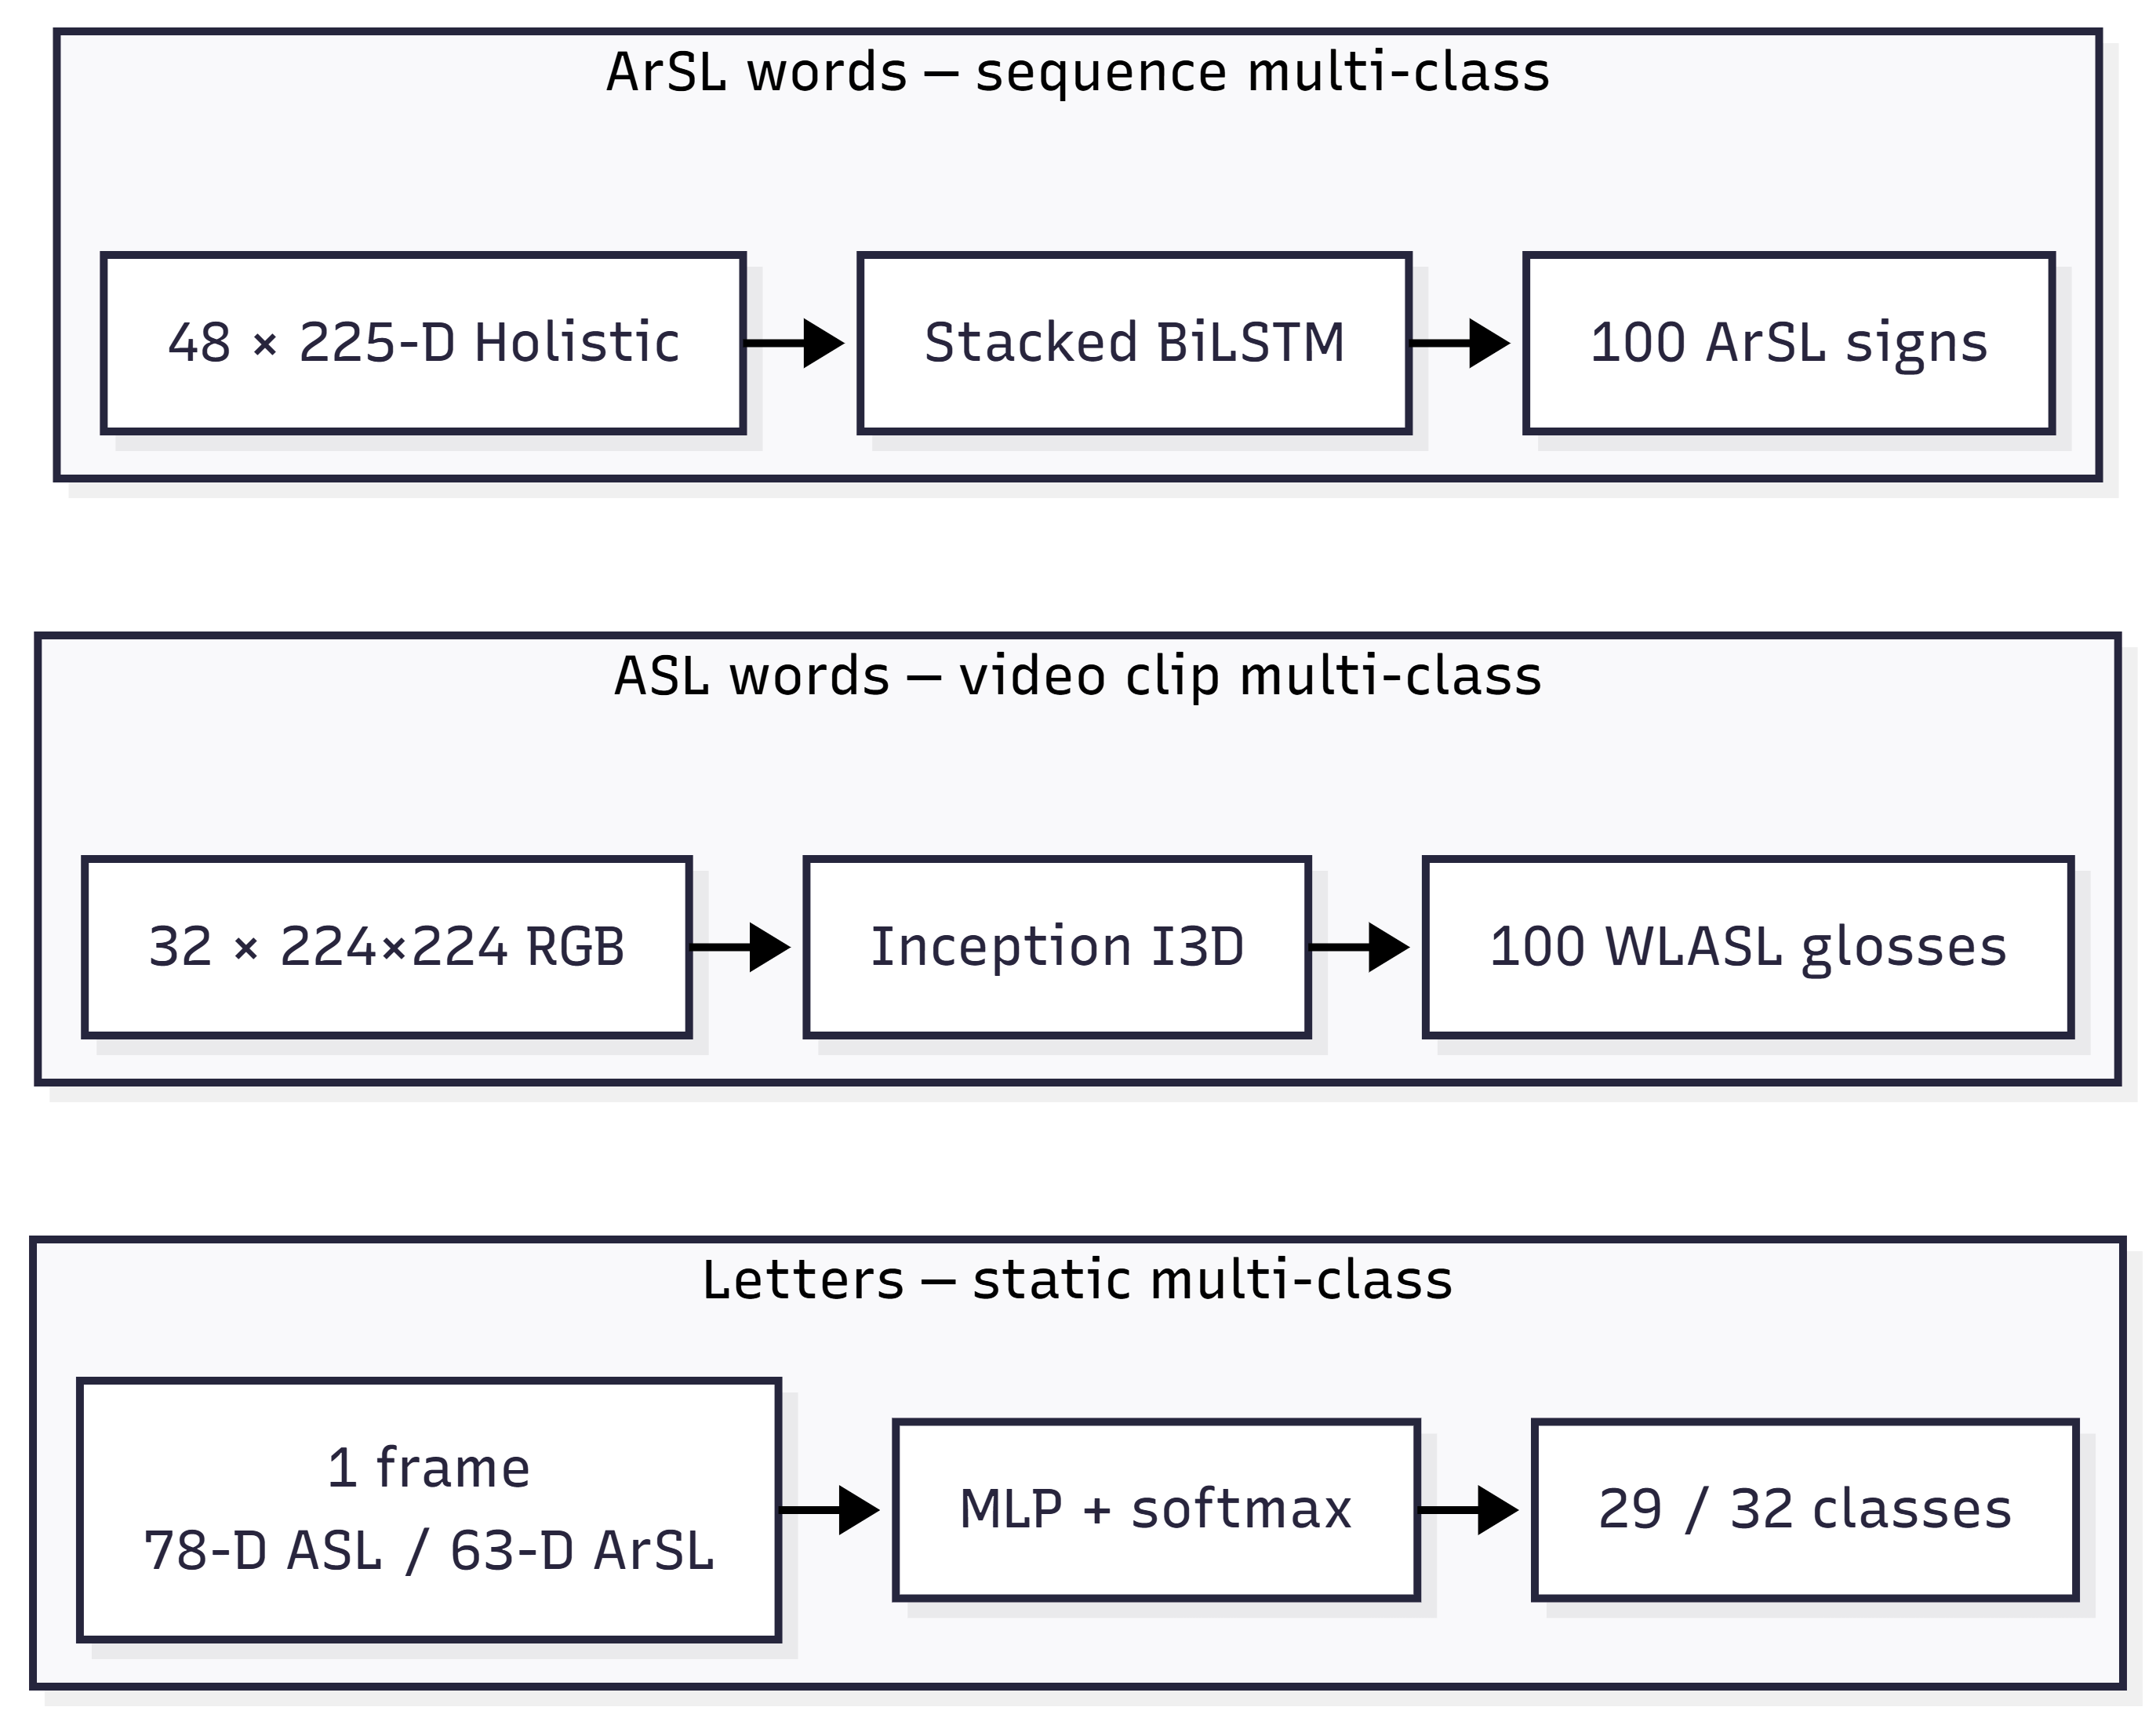
\includegraphics[width=0.95\textwidth]{images/fig_2-3_ml_paradigms.png}
\caption{Supervised machine-learning paradigms mapped to Eshara's four models (cf.\ Table~\ref{tab:ml-paradigms}): static MLPs for letters, Inception I3D for ASL words, and a stacked BiLSTM for ArSL words.}
\label{fig:ml-paradigms}
\end{figure}
\vspace{0.2cm}

\noindent As illustrated in Figure~\ref{fig:ml-paradigms}, input structure (single vector, RGB clip, or landmark sequence) determines the classifier family for each model. Full tensor shapes and training objectives are derived in Chapters~3 and~4.\par\vspace{0.2cm}

\noindent\textbf{2.2.3\quad Families of neural networks in SLR:}\par
\addcontentsline{toc}{subsection}{\numberline{2.2.3}Families of neural networks in SLR:}
\vspace{0.3cm}

\noindent Deep learning for SLR draws on several architectural families, each suited to a different input structure~\cite{adaloglou2022comprehensive,rastgoo2021survey}.\par\vspace{0.3cm}

\noindent \textbf{Multi-layer perceptrons (MLPs)} are feed-forward networks: information flows input $\rightarrow$ hidden layers $\rightarrow$ softmax output with no memory of previous frames. They are the standard choice when $T{=}1$ and latency must be minimal~\cite{ioffe2015batchnorm,srivastava2014dropout}.\par\vspace{0.3cm}

\noindent \textbf{Convolutional neural networks (CNNs)} apply learned filters over spatial dimensions (height $\times$ width of an image, or pseudo-spatial layouts of landmarks). CNNs dominated pixel-based SLR in the 2014--2018 period~\cite{he2016deep,sandler2018mobilenetv2}. Eshara uses CNNs in early letter-image experiments and in the deployed ASL word model (Inception I3D); letter models convert images to landmarks and train MLPs instead~\cite{zhang2020mediapipe,li2020wlasl}.\par\vspace{0.3cm}

\noindent \textbf{Recurrent neural networks (RNNs) and LSTMs} maintain a hidden state that is updated at each time step, allowing the model to aggregate information across frames. Long Short-Term Memory (LSTM) units avoid vanishing gradients on sequences of 32--48 frames~\cite{hochreiter1997long,pascanu2013difficulty}. Bidirectional LSTMs (BiLSTMs) read the sequence forward and backward so that both sign onset and completion inform the decision~\cite{schuster1997bidirectional,pigou2018sign}.\par\vspace{0.3cm}

\noindent \textbf{Attention mechanisms} learn which time steps (or feature subspaces) matter most for classification. Additive attention pools a weighted sum of BiLSTM outputs~\cite{bahdanau2015neural}; multi-head attention learns several attention patterns in parallel~\cite{vaswani2017attention}. Attention variants appear in the WLASL literature~\cite{li2020wlasl}; the ArSL word model uses a plain stacked BiLSTM without an explicit attention module~\cite{sidig2021karsl}.\par\vspace{0.3cm}

\noindent \textbf{Transformers} replace recurrence with self-attention over the full sequence. They achieve state-of-the-art results on large continuous SLR corpora but typically require more data and compute than BiLSTM models on graduation-scale vocabularies~\cite{vaswani2017attention,duarte2021how2sign}. Transformers are cited for context but are not the graduation architecture choice.\par\vspace{0.2cm}

\noindent\textbf{2.2.4\quad Training, validation, and evaluation:}\par
\addcontentsline{toc}{subsection}{\numberline{2.2.4}Training, validation, and evaluation:}
\vspace{0.3cm}

\noindent Supervised models are trained by minimising a \textbf{loss function} on labelled data. Eshara uses \textbf{categorical cross-entropy} for all four models: the network outputs a probability distribution over classes, and training penalises assignments that assign low probability to the correct label~\cite{szegedy2016rethinking,kingma2015adam}. Optimisation uses the Adam algorithm with mini-batches; dropout and batch normalisation reduce overfitting~\cite{kingma2015adam,ioffe2015batchnorm,srivastava2014dropout}.\par\vspace{0.2cm}

\noindent Data are partitioned into \textbf{training}, \textbf{validation}, and \textbf{test} sets. Training updates weights; validation selects hyperparameters and early-stopping checkpoints; test evaluation is run once on held-out data to report thesis metrics. Letter models use random image splits; the ArSL word model is evaluated on a held-out KArSL test partition (SignID 71--170)~\cite{sidig2021karsl}. Reporting validation accuracy alone would be optimistic; the thesis headline numbers are always \textbf{test-set} Top-1, Top-5 (word models), and macro-F1~\cite{li2020wlasl,rastgoo2021survey}.\par\vspace{0.2cm}

\noindent The following table summarises evaluation metrics common in the SLR literature and explains which Eshara reports in Chapter~6. Word models with imbalanced or scarce per-class data benefit from Top-5 and macro-F1 in addition to Top-1~\cite{li2020wlasl,sidig2021karsl}.\par\vspace{0.2cm}

\begin{table}[H]
\centering
\caption{Evaluation metrics in SLR literature and in Eshara.}
\label{tab:eval-metrics}
\small
\begin{tabular}{|P{2.8cm}|P{3.2cm}|P{3.0cm}|}
\hline
\multicolumn{1}{|c|}{\textbf{Metric}} & \multicolumn{1}{|c|}{\textbf{Typical use in SLR}} & \multicolumn{1}{|c|}{\textbf{Eshara usage}}\\
\hline
Top-1 accuracy & Isolated classification & All four models (headline) \\
\hline
Top-5 accuracy & Large / imbalanced vocabularies & ASL + ArSL word models \\
\hline
Macro-F1 & Per-class balance (scarce classes) & Word models; ArSL graduation headline \\
\hline
Weighted-F1 & Sample-frequency weighting & Reported alongside macro-F1 (ArSL) \\
\hline
WER / CER & Continuous SLR, translation & Not used (isolated scope) \\
\hline
Signer-independent acc. & Generalisation across signers & Future work; held-out clip splits for word models \\
\hline
\end{tabular}
\end{table}
\vspace{0.2cm}

\noindent\textbf{2.2.5\quad Isolated SLR versus continuous SLR as ML problems:}\par
\addcontentsline{toc}{subsection}{\numberline{2.2.5}Isolated SLR versus continuous SLR as ML problems:}
\vspace{0.3cm}

\noindent It is useful to distinguish two \textbf{problem formulations} in the literature. \emph{Isolated sign recognition} is standard multi-class classification: each clip contains one known sign, and the model outputs one label. \emph{Continuous sign recognition} is sequence-to-sequence learning: an unsegmented video may contain many signs, and the model must output a sequence of gloss labels with correct boundaries~\cite{koller2020weakly,camgoz2018neural}. Continuous SLR additionally requires \textbf{segmentation} (detecting where one sign ends) and often \textbf{language modelling} across glosses. Eshara solves only the isolated formulation: the user pauses between signs, and the web UI buffers one letter pose or one word motion window at a time. This reduces problem complexity and matches the educational and assistive use cases targeted in graduation scope~\cite{li2020wlasl,sidig2021karsl,duarte2021how2sign}.\par\vspace{0.2cm}

\begin{figure}[H]
\centering
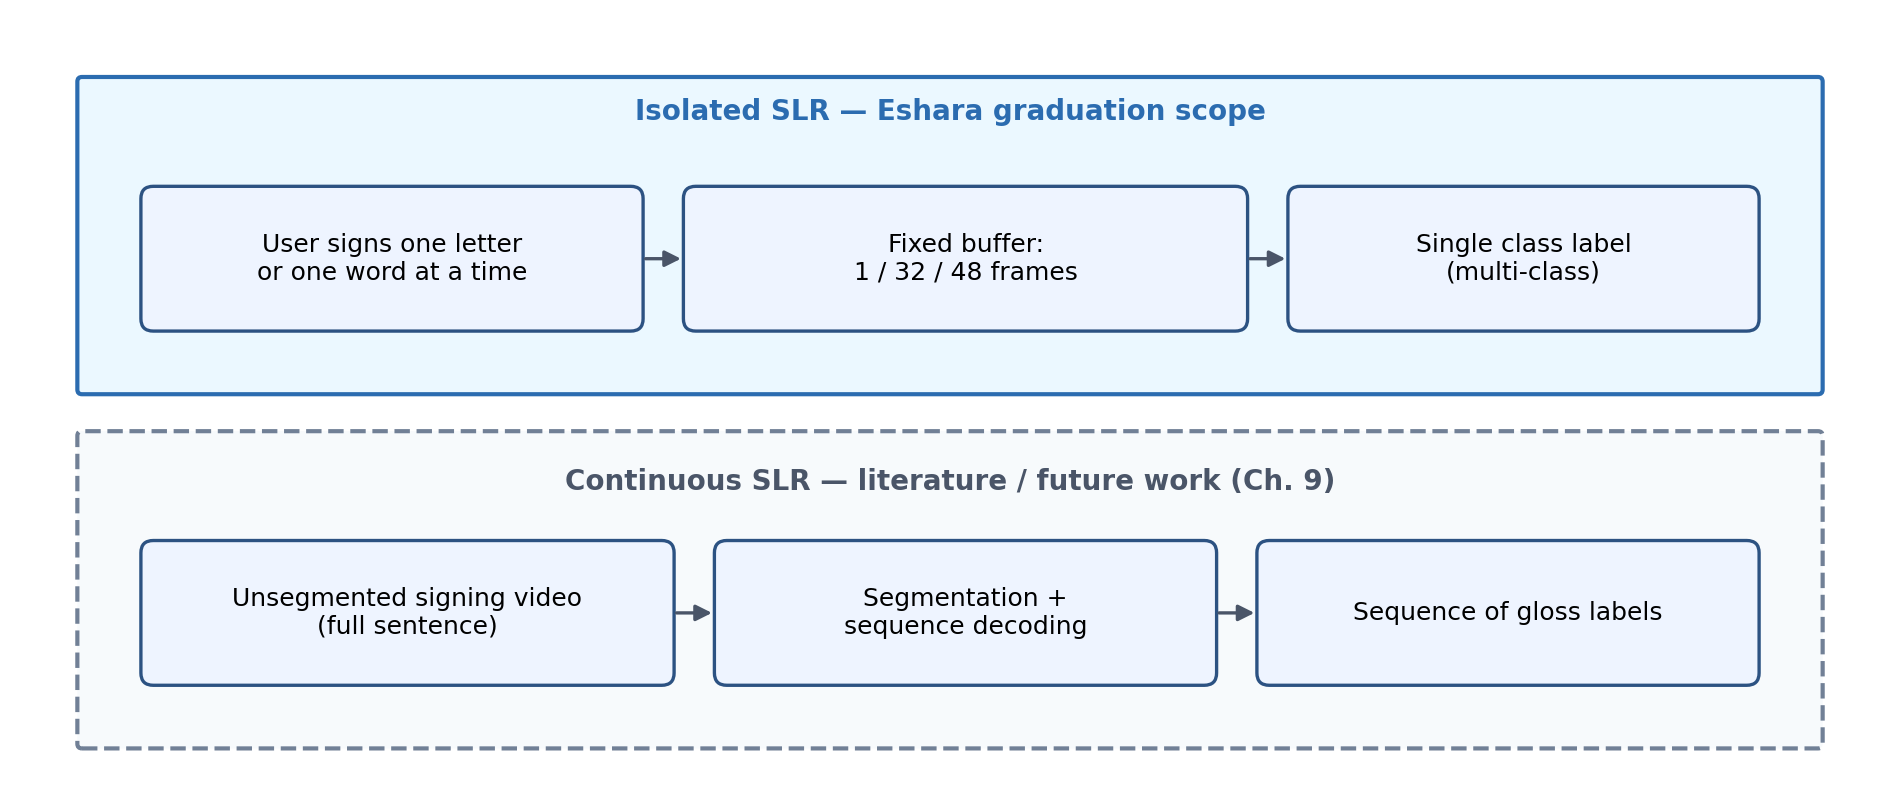
\includegraphics[width=0.88\textwidth]{images/fig_2-4_isolated_vs_continuous.png}
\caption{Isolated versus continuous sign-language recognition as machine-learning problem formulations. Eshara implements isolated classification only; continuous gloss decoding is deferred to Chapter~9.}
\label{fig:isolated-vs-continuous}
\end{figure}
\vspace{0.2cm}

\noindent As illustrated in the following figure, the fixed-buffer interaction model used in Eshara contrasts with the segmentation and sequence-decoding requirements of continuous SLR benchmarks such as How2Sign and RWTH-PHOENIX~\cite{duarte2021how2sign,forster2014rwth}.\par\vspace{0.2cm}

\noindent\textbf{2.2.6\quad Preprocessing, normalisation, and augmentation:}\par
\addcontentsline{toc}{subsection}{\numberline{2.2.6}Preprocessing, normalisation, and augmentation:}
\vspace{0.3cm}

\noindent Landmark-based SLR pipelines share a common preprocessing stage before neural classification~\cite{zhang2020mediapipe,deng2024skeleton,adaloglou2022comprehensive}. Landmarks are typically \textbf{centred} on a reference joint (wrist or shoulder) and \textbf{scale-normalised} by inter-joint distance so that signer height and camera distance have reduced influence. \textbf{Missing} detections from occlusion are zero-filled or linearly interpolated; the live web client applies the same convention as offline training for consistency~\cite{zhang2020mediapipe}. \textbf{Standardisation} (subtract training mean, divide by training standard deviation per feature dimension) is common in the literature and is fit on the training split only to prevent test leakage; Eshara's letter MLPs and deployed word models instead rely on geometric normalisation and in-network batch normalisation without external \texttt{StandardScaler} checkpoints (Chapters~3--4).\par\vspace{0.3cm}

\noindent \textbf{Data augmentation} is widely used when per-class sample counts are low~\cite{perez2017augmentation,sidig2021karsl}. Image-based SLR applies spatial transforms (rotation, crop, colour jitter) to hand crops; sequence-based SLR may apply temporal jitter, frame dropout, or additive noise on landmark trajectories. Letter models rely on large balanced image corpora; ASL word I3D uses pretrained WLASL weights with standard frame-level normalisation at inference.\par\vspace{0.3cm}
\clearpage
% --- 2.3 COMPUTER VISION APPROACHES ---
\noindent\textbf{2.3\quad COMPUTER VISION APPROACHES TO SLR}\par
\addcontentsline{toc}{section}{\numberline{2.3}COMPUTER VISION APPROACHES TO SLR}
\vspace{0.2cm}

\noindent\textbf{2.3.1\quad Image-Based Convolutional Methods:}\par
\addcontentsline{toc}{subsection}{\numberline{2.3.1}Image-Based Convolutional Methods:}
\vspace{0.3cm}

\noindent Deep convolutional networks such as ResNet~\cite{he2016deep}, MobileNetV2~\cite{sandler2018mobilenetv2,howard2017mobilenets}, and EfficientNet~\cite{tan2019efficientnet} established strong baselines for image classification by learning spatial hierarchies of visual features. Several sign-language studies apply similar architectures to hand images or signing clips, reporting high accuracy when camera viewpoint, background, and signer identity are constrained~\cite{rastgoo2021survey,pigou2018sign,huang2018attention}. Residual connections~\cite{he2016deep} ease optimisation of deep stacks; inverted residuals and depthwise separable convolutions~\cite{sandler2018mobilenetv2} reduce multiply--accumulate cost, which is attractive for edge deployment. EfficientNet~\cite{tan2019efficientnet} further trades off depth, width, and resolution through compound scaling.\par\vspace{0.2cm}

\noindent Despite strong offline metrics, three limitations motivate Eshara's \textbf{hybrid input design} for live webcam use. \textbf{Generalisation:} a model trained on cropped dataset images may degrade on new backgrounds, skin tones, jewellery, or lower-resolution webcams because pixel statistics shift while kinematic structure remains stable~\cite{zhang2020mediapipe}. \textbf{Compute:} letter and ArSL word paths classify compact landmark vectors (63--225 dimensions per frame) on modest hardware, whereas ASL word I3D requires batched 3D convolutions on 32-frame RGB clips~\cite{sandler2018mobilenetv2,li2020wlasl}. \textbf{Pipeline mismatch:} if training uses static dataset photographs but inference uses a live camera, the system must solve two domain-shift problems simultaneously (vision appearance and temporal sampling) rather than one (landmark noise only).\par\vspace{0.2cm}

\noindent The following table records vision pipelines explored during development and the rationale for the graduation choice. During early experimentation, MobileNetV2 was trained on hand-cropped letter images. Although accuracy on fixed-view dataset images was competitive, the domain gap between curated photographs and live webcam capture motivated a unified landmark representation instead. Eshara's letter pipelines illustrate this pragmatic compromise. The ASL and ArSL letter corpora are distributed as static hand images~\cite{akash2019aslalphabet,arthur2018arasl2018}, yet both are converted offline to MediaPipe hand landmarks --- 78-D engineered vectors for ASL and 63-D raw vectors for ArSL --- and trained with the same MLP \emph{architectural family} but language-specific hidden widths and hyperparameters (Chapter~3). At runtime the same feature conventions are preserved through the deployed inference path, reducing train--serve drift. This design follows the broader literature consensus that skeleton features narrow the domain gap between curated datasets and casual camera capture~\cite{zhang2020mediapipe,rastgoo2021survey,adaloglou2022comprehensive,deng2024skeleton}.\par\vspace{0.2cm}

\begin{table}[H]
\centering
\caption{Vision pipelines considered during Eshara development.}
\label{tab:approaches-considered}
\small
\begin{tabular}{|P{2.8cm}|P{3.2cm}|P{3.0cm}|}
\hline
\multicolumn{1}{|c|}{\textbf{Approach}} & \multicolumn{1}{|c|}{\textbf{Explored in project?}} & \multicolumn{1}{|c|}{\textbf{Outcome}}\\
\hline
Sensor gloves / Kinect depth & No (graduation scope) & Historical; not deployable on standard webcams \\
\hline
MobileNetV2 on hand images & Yes (early trials) & Strong offline; webcam domain gap \\
\hline
Pixel CNN / ResNet on video & Limited trials & Heavy; mismatched live pipeline \\
\hline
Landmarks + MLP (letters) & \textbf{Yes --- deployed} & Unified train/live representation \\
\hline
I3D on RGB (ASL words) & \textbf{Yes --- deployed} & 32-frame video clips \\
\hline
Landmarks + BiLSTM (ArSL words) & \textbf{Yes --- deployed} & 48-frame sequences \\
\hline
Full Transformer on words & Trial experiments & VRAM/data limits on graduation GPU \\
\hline
Single multilingual model & No & Incompatible label spaces (EN$\neq$AR) \\
\hline
\end{tabular}
\end{table}
\vspace{0.2cm}

\noindent\textbf{2.3.2\quad Skeleton and Landmark Methods:}\par
\addcontentsline{toc}{subsection}{\numberline{2.3.2}Skeleton and Landmark Methods:}
\vspace{0.3cm}

\noindent MediaPipe Hands uses a two-stage pipeline: a palm detector proposes hand regions, and a landmark regressor outputs 21 three-dimensional points per hand in normalised image coordinates~\cite{zhang2020mediapipe}. Each point carries $(x,y,z)$ relative to the hand bounding box, yielding $21 \times 3 = 63$ values per frame per hand. For finger-spelling, this single-frame vector is sufficient because letter signs are quasi-static poses: the classifier decision depends on fingertip configuration rather than long-horizon motion~\cite{akash2019aslalphabet,arthur2018arasl2018}. Word signs, by contrast, involve trajectory, two-handed coordination, facial grammar, and upper-body motion~\cite{li2020wlasl,sidig2021karsl}. Eshara therefore uses three feature regimes matched to task complexity, summarised in Table~\ref{tab:feature-vectors}.\par\vspace{0.2cm}

\begin{table}[H]
\centering
\caption{Feature-vector composition used by each Eshara model.}
\label{tab:feature-vectors}
\small
\begin{tabular}{|P{2.6cm}|r|r|r|P{3.8cm}|}
\hline
\multicolumn{1}{|c|}{\textbf{Model}} & \multicolumn{1}{|c|}{\textbf{Dim./frame}} & \multicolumn{1}{|c|}{\textbf{Frames}} & \multicolumn{1}{|c|}{\textbf{Tensor shape}} & \multicolumn{1}{|c|}{\textbf{Input source}}\\
\hline
ASL Letter MLP & 78 & 1 & $(78,)$ & MediaPipe Hands (engineered) \\
\hline
ArSL Letter MLP & 63 & 1 & $(63,)$ & MediaPipe Hands (raw) \\
\hline
ASL Word I3D & 224$\times$224 RGB & 32 & $(32, 224, 224, 3)$ & Raw webcam frames \\
\hline
ArSL Word BiLSTM & 225 & 48 & $(48, 225)$ & MediaPipe Holistic (normalised) \\
\hline
\end{tabular}
\end{table}
\vspace{0.2cm}

\noindent The ASL word model (Inception I3D) does not use landmarks: it consumes \textbf{raw RGB frames} ($32 \times 224 \times 224 \times 3$) normalised to $[-1,1]$. No MediaPipe extraction is required at inference time; the client buffers 32 centre-cropped frames and transmits them as encoded image data~\cite{li2020wlasl,zhang2020mediapipe}. The ArSL word model uses a \textbf{225-dimensional} normalised Holistic vector per frame: body pose ($33 \times 3 = 99$) centred on the nose, left hand ($21 \times 3 = 63$) centred on its wrist, and right hand ($21 \times 3 = 63$) centred on its wrist, giving $99 + 63 + 63 = 225$~\cite{sidig2021karsl,bazarevsky2020blazepose}. This body-relative normalisation reduces sensitivity to signer distance and height. The 48-frame window reflects the average sign duration in KArSL word clips~\cite{sidig2021karsl}.\par\vspace{0.2cm}

\noindent Before model input, landmarks are centred and scale-normalised (typically relative to wrist or shoulder width) so that signer body size and distance from the camera have reduced influence. Missing landmarks from occlusion are zero-filled or interpolated in the training pipeline; the deployed inference services apply the same convention for consistency~\cite{zhang2020mediapipe}. Landmark pipelines offer three engineering advantages emphasised in the literature but rarely demonstrated together in deployed bilingual systems. First, they require less labelled video than pixel-level models because the input dimensionality is orders of magnitude smaller~\cite{rastgoo2021survey,adaloglou2022comprehensive}. Second, they support privacy-preserving designs on letter and ArSL word paths: compact features are processed per request, while ASL word mode sends encoded frame buffers instead of continuous raw video. Third, MediaPipe provides runtimes suitable for real-time extraction in practical web systems~\cite{mediapipeweb,zhang2020mediapipe}.\par\vspace{0.2cm}

\noindent OpenPose remains a widely cited baseline but is heavier and lacks a first-class browser runtime~\cite{cao2019openpose}. MediaPipe Holistic (543 raw landmarks) and MoveNet (17 body keypoints) were evaluated during development; Holistic proved too slow for sustained live word recognition on laptop hardware at the target frame rate, while MoveNet lacks the dual-hand detail required for finger-spelling~\cite{yu2021movenet,bazarevsky2020blazepose}. as compared in Table~\ref{tab:pose-frameworks} (Section~2.5), which compares these frameworks quantitatively.\par\vspace{0.2cm}

\begin{figure}[H]
\centering
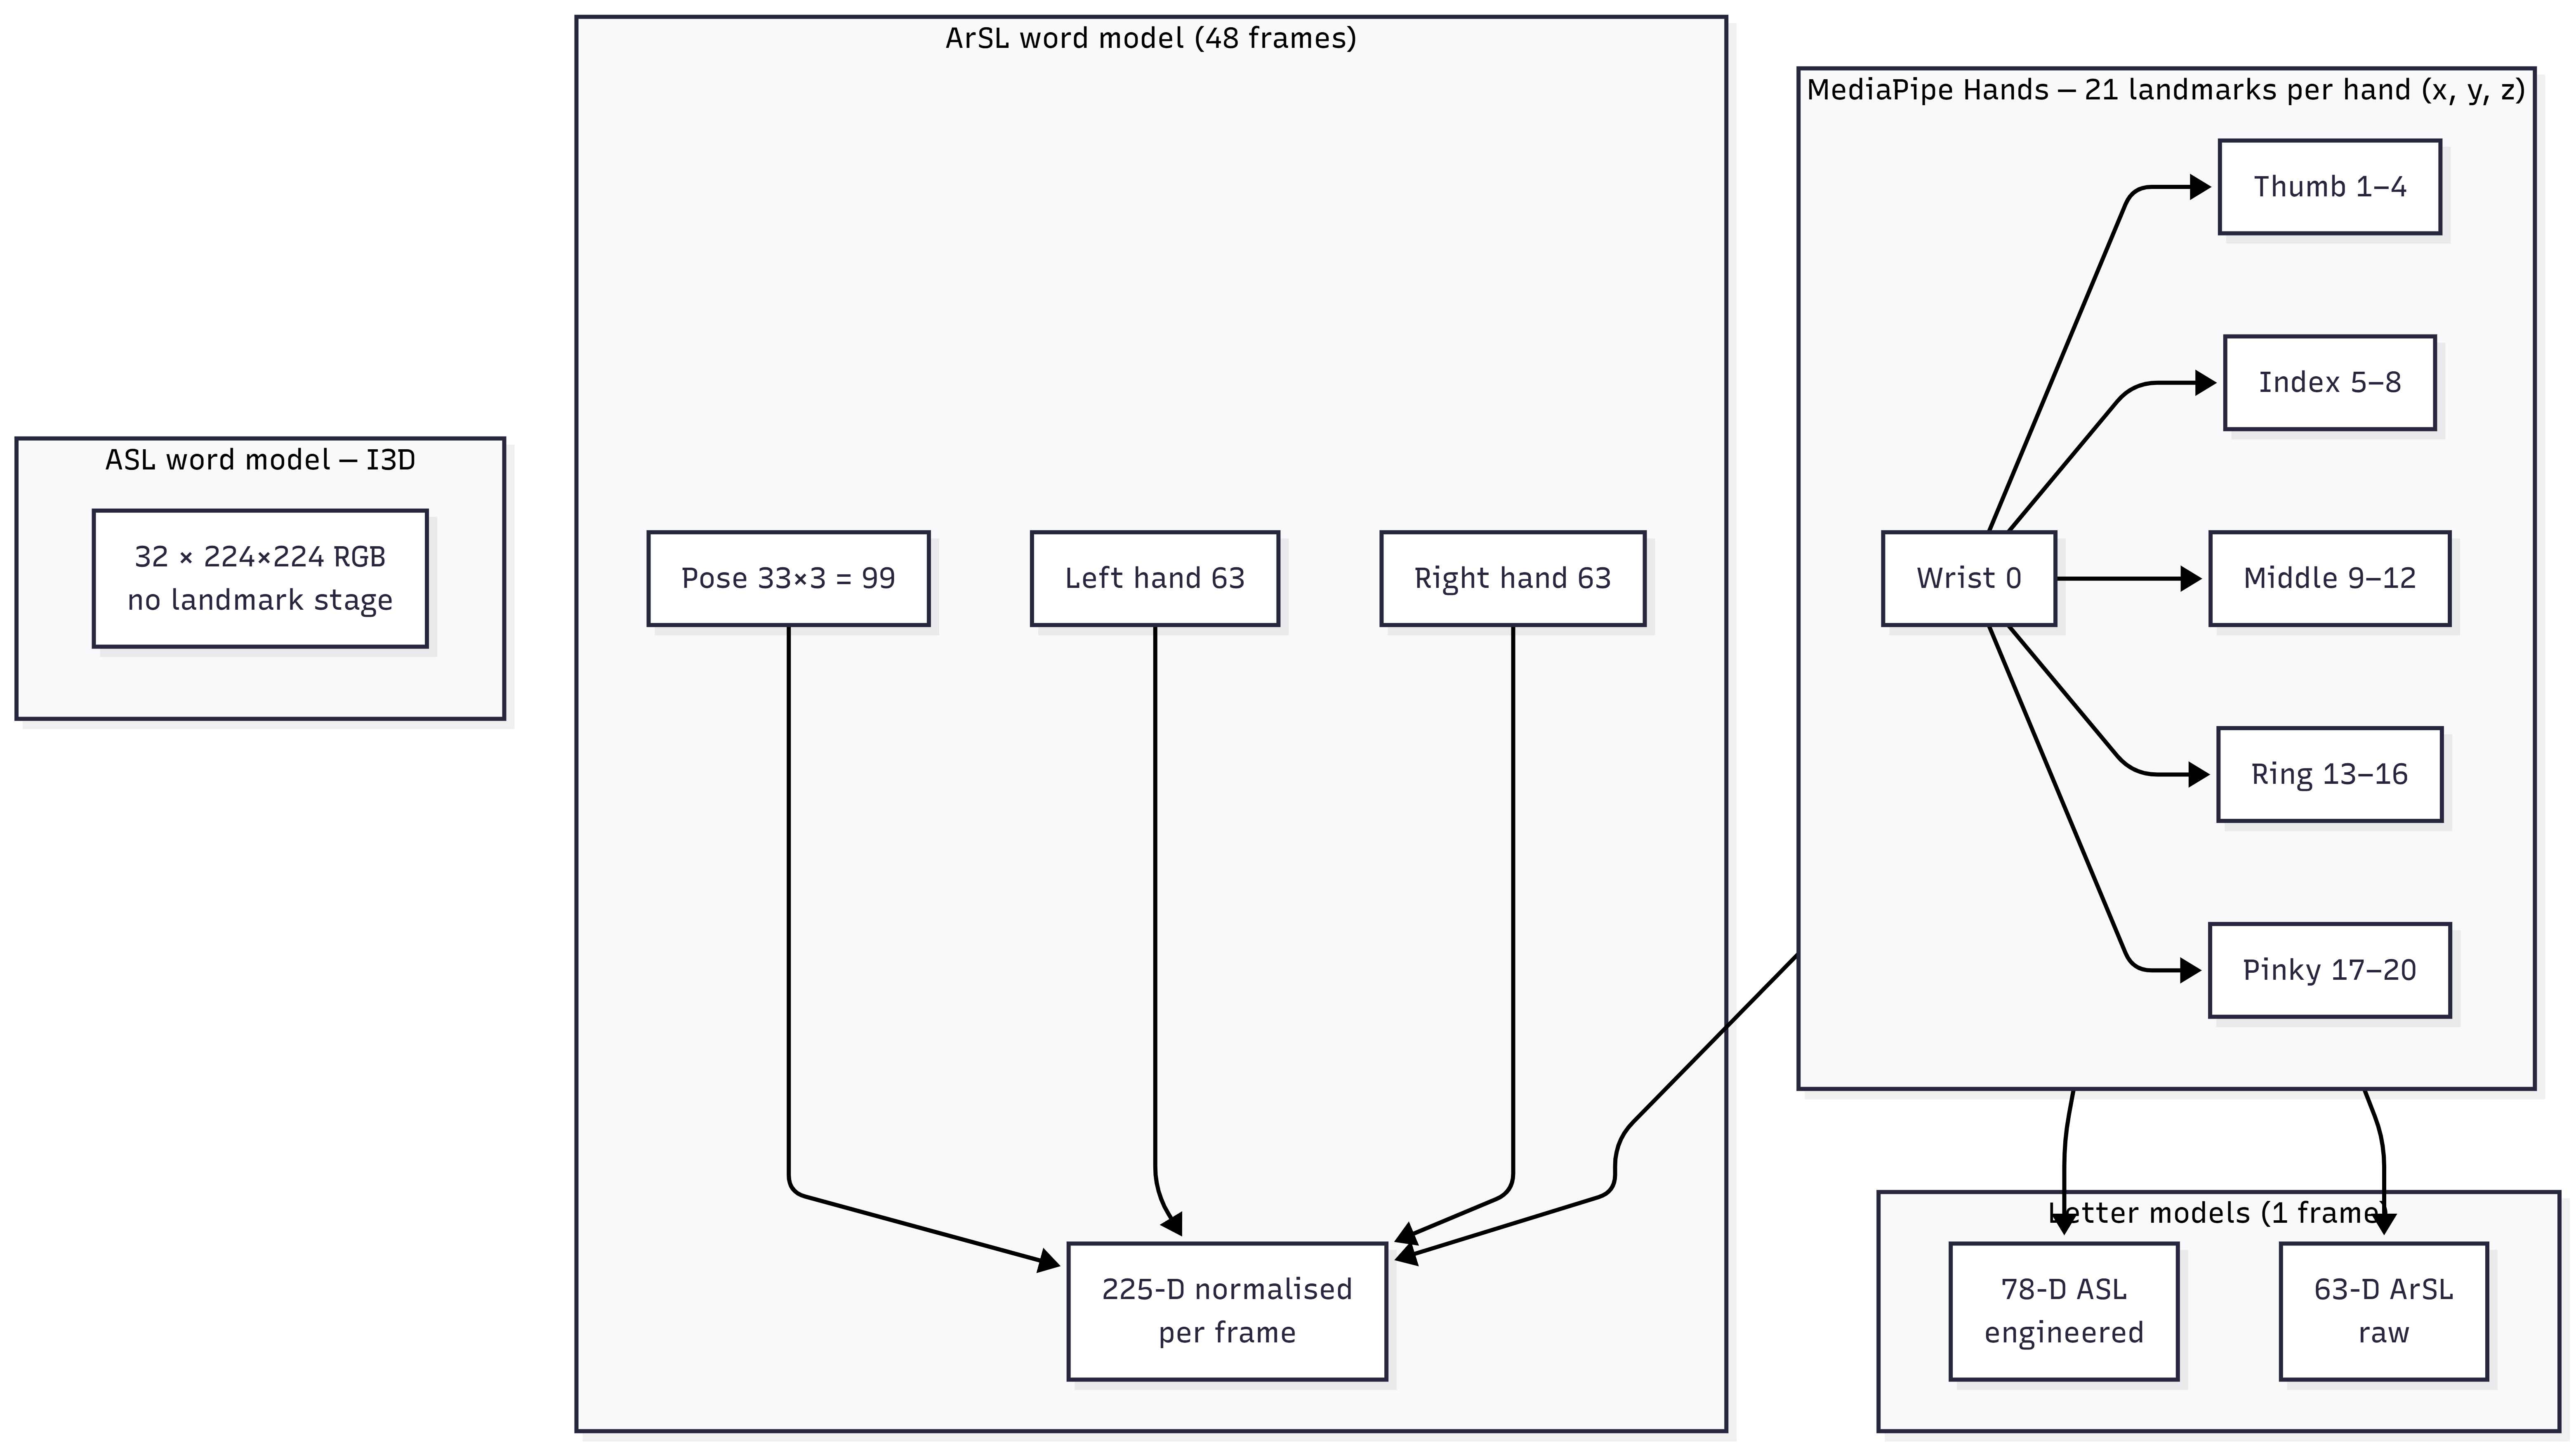
\includegraphics[width=0.88\textwidth]{images/fig_2-2_hand_landmarks.png}
\caption{MediaPipe hand landmarks (63-D per frame) and extension to normalised pose+hands feature vectors used by the ArSL word model (225-D). The ASL word model (I3D) consumes raw RGB frames rather than landmarks.}
\label{fig:hand-landmarks}
\end{figure}
\vspace{0.2cm}

\noindent As illustrated in Figure~\ref{fig:hand-landmarks}, finger-spelling needs only the 21-point hand mesh, whereas ArSL word recognition concatenates body pose and both hands into a 225-D normalised vector per frame. ASL word recognition bypasses landmarks entirely and feeds raw RGB clips into a pretrained I3D network~\cite{zhang2020mediapipe,bazarevsky2020blazepose,mediapipeweb,li2020wlasl}.\par\vspace{0.2cm}

\noindent\textbf{2.3.3\quad Hybrid CNN--RNN and Continuous SLR:}\par
\addcontentsline{toc}{subsection}{\numberline{2.3.3}Hybrid CNN--RNN and Continuous SLR:}
\vspace{0.3cm}

\noindent For sentence-level tasks, the dominant pattern is a visual encoder followed by a sequence model. Neural sign-language translation (SLT) systems pair convolutional front ends with recurrent or attention decoders to map signing video to spoken-language text without an intermediate gloss step in some architectures~\cite{camgoz2018neural}. Weakly supervised continuous sign-language recognition (CSLR) further shows that gloss-level alignment can be learned from untrimmed broadcast footage when only sentence-level weak labels are available~\cite{koller2020weakly}. Large-scale benchmarks such as How2Sign provide hundreds of hours of continuous American Sign Language aligned with English subtitles for this research line~\cite{duarte2021how2sign}, while RWTH-PHOENIX-Weather serves a similar role for German Sign Language~\cite{forster2014rwth}.\par\vspace{0.2cm}

\noindent Continuous systems must solve \emph{segmentation} (where one sign ends and the next begins) in addition to \emph{classification} (which sign is being performed). Isolated classifiers sidestep segmentation by asking the user to pause between signs --- a deliberate interaction pattern suitable for a graduation web demo and for educational finger-spelling practice. Eshara word models therefore classify fixed-length inputs --- 32-frame RGB clips for ASL words or 48-frame landmark sequences for ArSL words --- into a closed vocabulary rather than decoding unbounded gloss sequences. This is a well-studied stepping stone toward sentence-level systems and matches the interaction model of a user deliberately signing one word at a time in front of a webcam~\cite{li2020wlasl,sidig2021karsl,pigou2018sign}.\par\vspace{0.3cm}

% --- 2.4 DEEP-LEARNING ARCHITECTURES ---
\noindent\textbf{2.4\quad DEEP-LEARNING ARCHITECTURES}\par
\addcontentsline{toc}{section}{\numberline{2.4}DEEP-LEARNING ARCHITECTURES}
\vspace{0.2cm}

\noindent The four Eshara models span three architectural families introduced in Section~2.2: feed-forward MLPs for static letters, a 3D CNN (Inception I3D) for ASL words, and a stacked BiLSTM for ArSL words. This section states each family at a \textbf{conceptual} level only --- enough to follow the literature review. Full tensor layouts, layer dimensions, normalisation steps, loss functions, and training protocols are derived in Chapter~3 (letters) and Chapter~4 (words).\par\vspace{0.2cm}

\noindent\textbf{2.4.1\quad Multi-Layer Perceptrons (letter models):}\par
\addcontentsline{toc}{subsection}{\numberline{2.4.1}Multi-Layer Perceptrons (letter models):}
\vspace{0.3cm}

\noindent An MLP maps a single input vector $\mathbf{x}$ to a class label through a stack of fully connected layers. Each hidden layer applies an affine transform followed by a non-linear activation (ReLU in Eshara), optionally with batch normalisation and dropout for regularisation~\cite{ioffe2015batchnorm,srivastava2014dropout}. The final layer outputs a score vector $\mathbf{z}$ over $C$ classes; softmax converts these scores into a probability distribution and the predicted class is $\hat{y} = \arg\max_k P(y{=}k \mid \mathbf{x})$~\cite{szegedy2016rethinking}. Because finger-spelled letters are quasi-static poses, no recurrence is required: one 78-D (ASL) or 63-D (ArSL) vector per frame suffices. Chapter~3 specifies the exact layer widths ($256 \rightarrow 128 \rightarrow 64 \rightarrow C$ for ASL; $512 \rightarrow 256 \rightarrow 64 \rightarrow C$ for ArSL), the ASL 78-D feature-engineering equations, batch-norm and dropout placement, the cross-entropy loss, and the $\sim$49\,k / $\sim$183\,k parameter counts for Models~1 and~2.\par\vspace{0.2cm}

\noindent\textbf{2.4.2\quad Inception I3D (ASL word model):}\par
\addcontentsline{toc}{subsection}{\numberline{2.4.2}Inception I3D (ASL word model):}
\vspace{0.3cm}

\noindent Inception I3D (Inflated 3D ConvNet) extends 2D Inception modules to video by convolving jointly over spatial height, width, and time~\cite{li2020wlasl}. The ASL word model consumes a clip of $T{=}32$ centre-cropped RGB frames ($224 \times 224$ per frame), learns spatio-temporal filters without hand-crafted landmarks, and outputs logits over 100 WLASL glosses. Per-frame predictions are averaged over time before argmax classification. Eshara deploys a pretrained Inception I3D checkpoint (\texttt{asl\_word\_i3d.pt}) rather than training from scratch within graduation GPU limits. Chapter~4 documents clip buffering, $[-1,1]$ frame normalisation, and the Model~3 architecture; Chapter~5 documents the live web pipeline.\par\vspace{0.2cm}

\noindent\textbf{2.4.3\quad Bidirectional LSTM (ArSL word model):}\par
\addcontentsline{toc}{subsection}{\numberline{2.4.3}Bidirectional LSTM (ArSL word model):}
\vspace{0.3cm}

\noindent A Long Short-Term Memory (LSTM) network maintains a hidden state that is updated at each time step, allowing the model to aggregate motion across a signing clip~\cite{hochreiter1997long,pascanu2013difficulty}. Gated units control how much past context is retained or forgotten at each frame. A \textbf{bidirectional} LSTM reads the sequence forward and backward and concatenates both hidden states at each step, so sign onset and completion both inform the final decision~\cite{schuster1997bidirectional,pigou2018sign}. The ArSL word model stacks two BiLSTM layers on 48-frame sequences of 225-D normalised Holistic vectors and classifies into 100 Arabic sign classes with a dense softmax head; no explicit attention module is used. Chapter~4 gives the full gate equations, tensor shapes $(48, 225)$, nose/wrist normalisation, and evaluation on the held-out KArSL test partition (SignID 71--170).\par\vspace{0.2cm}

\noindent\textbf{2.4.4\quad Attention and transformers (literature context):}\par
\addcontentsline{toc}{subsection}{\numberline{2.4.4}Attention and transformers (literature context):}
\vspace{0.3cm}

\noindent \textbf{Attention} mechanisms learn which time steps in a clip carry the most discriminative motion --- useful when neutral rest frames precede or follow the stroke phase~\cite{bahdanau2015neural,li2020wlasl,huang2018attention}. Additive and multi-head variants appear in the WLASL literature but are \textbf{not} part of Eshara's graduation architectures. \textbf{Transformers} replace recurrence with self-attention over the full sequence and achieve strong results on large continuous-SLR corpora, but typically require more data and compute than BiLSTM or I3D models at graduation vocabulary scale~\cite{vaswani2017attention,duarte2021how2sign}. They are cited here for context only.\par\vspace{0.3cm}

% --- 2.5 POSE ESTIMATION (TABLE) ---
\noindent\textbf{2.5\quad POSE-ESTIMATION FRAMEWORKS}\par
\addcontentsline{toc}{section}{\numberline{2.5}POSE-ESTIMATION FRAMEWORKS}
\vspace{0.2cm}

\noindent The following table compares frameworks considered for Eshara. Selection criteria were: (i)~availability of a maintained browser/WASM build; (ii)~sustained $\geq$25\,FPS on a mid-range laptop webcam stream; (iii)~compatibility with dual-hand finger-spelling; and (iv)~sufficient body keypoints for ArSL word motion~\cite{zhang2020mediapipe,bazarevsky2020blazepose,mediapipeweb,cao2019openpose}.\par\vspace{0.2cm}

\begin{table}[H]
\centering
\caption{Comparison of pose-estimation frameworks.}
\label{tab:pose-frameworks}
\small
\begin{tabular}{|P{2.5cm}|c|c|c|P{4.8cm}|}
\hline
\multicolumn{1}{|c|}{\textbf{Framework}} & \multicolumn{1}{|c|}{\textbf{Landmarks}} & \multicolumn{1}{|c|}{\textbf{Typical FPS}} & \multicolumn{1}{|c|}{\textbf{Browser}} & \multicolumn{1}{|c|}{\textbf{Role in Eshara}}\\
\hline
MediaPipe Hands & 21 per hand & 30+ & Yes (WASM) & Letter models (78-D ASL / 63-D ArSL) \\
\hline
MediaPipe Holistic & 543 & 18 & Yes & Literature reference; ASL word uses I3D (raw RGB) \\
\hline
MediaPipe Pose + Hands & 33 + 21$\times$2 & 25+ & Yes (WASM) & ArSL word model (225-D normalised) \\
\hline
OpenPose & 25 body & 8 & No & Literature baseline \\
\hline
MoveNet & 17 & 40+ & Yes & Compared, not used \\
\hline
\end{tabular}
\end{table}
\vspace{0.2cm}

\noindent MediaPipe Hands satisfies real-time letter recognition with the lowest feature dimensionality. Holistic provides the richest context for ASL words but at higher per-frame cost; it is used offline and in the browser word mode where the user holds still briefly during a sign. Pose+Hands offers the best balance for ArSL graduation words: full torso and dual-hand coverage without the face mesh overhead. OpenPose is included as a historical baseline from the literature~\cite{cao2019openpose} but was not integrated because deployment targets the browser, not a C++ desktop server. MoveNet's 17-point skeleton is insufficient for distinguishing ArSL two-hand minimal pairs~\cite{yu2021movenet,sidig2021karsl}.\par\vspace{0.3cm}

% --- 2.6 DATASETS (TABLE) ---
\noindent\textbf{2.6\quad SIGN-LANGUAGE DATASETS}\par
\addcontentsline{toc}{section}{\numberline{2.6}SIGN-LANGUAGE DATASETS}
\vspace{0.2cm}

\noindent The following table summarises the corpora that ground the four Eshara models. A deliberate design constraint is that \textbf{each model maintains its own label space}; vocabularies are not shared across languages or tasks~\cite{li2020wlasl,sidig2021karsl}. This avoids impossible label alignment (an ASL gloss does not correspond to an ArSL gloss) and allows independent retraining when one corpus is updated.\par\vspace{0.2cm}

\begin{table}[H]
\centering
\caption{Sign-language datasets used or referenced in this work.}
\label{tab:datasets}
\small
\begin{tabular}{|P{2.4cm}|c|c|r|r|P{3.5cm}|}
\hline
\multicolumn{1}{|c|}{\textbf{Dataset}} & \multicolumn{1}{|c|}{\textbf{Lang.}} & \multicolumn{1}{|c|}{\textbf{Type}} & \multicolumn{1}{|c|}{\textbf{Classes}} & \multicolumn{1}{|c|}{\textbf{Samples}} & \multicolumn{1}{|c|}{\textbf{Role}}\\
\hline
ASL Alphabet (Kaggle) & ASL & Images & 29 & 87\,000 & ASL letter MLP \\
\hline
ArASL2018 & ArSL & Images & 32 & 54\,049 & ArSL letter MLP \\
\hline
WLASL-2000 & ASL & Video & 2000 & 21\,000 & 100-class I3D subset \\
\hline
KArSL-502 & ArSL & Video & 502 & 24\,000 & 100-class word subset (SignID 71--170) \\
\hline
How2Sign & ASL & Continuous & --- & 80\,h & Future work (Ch.~8) \\
\hline
RWTH-PHOENIX & DGS & Continuous & --- & --- & Comparison only \\
\hline
\end{tabular}
\end{table}
\vspace{0.2cm}

\noindent The following table highlights \textbf{class imbalance} and average samples per class --- a key reason Eshara reports macro-F1 and Top-5 for word models, uses a 100-class WLASL subset for I3D, and a 100-class KArSL word subset for the ArSL BiLSTM~\cite{li2020wlasl,sidig2021karsl}.\par\vspace{0.2cm}

\begin{table}[H]
\centering
\caption{Approximate class balance across Eshara training corpora.}
\label{tab:dataset-imbalance}
\small
\begin{tabular}{|P{2.8cm}|r|r|r|P{3.5cm}|}
\hline
\multicolumn{1}{|c|}{\textbf{Corpus (Eshara use)}} & \multicolumn{1}{|c|}{\textbf{Classes}} & \multicolumn{1}{|c|}{\textbf{Total samples}} & \multicolumn{1}{|c|}{\textbf{$\sim$Avg/class}} & \multicolumn{1}{|c|}{\textbf{Implication}}\\
\hline
ASL Alphabet & 29 & 87\,000 & $\sim$3\,000 & Balanced; Top-1 sufficient \\
\hline
ArASL2018 & 32 & 54\,049 & $\sim$1\,700 & Balanced; more confusion pairs \\
\hline
WLASL I3D subset & 100 & $\sim$3\,000 clips & 10--50 (varies) & I3D pretrained; Top-5 \\
\hline
KArSL word subset & 100 & $\sim$4\,800 seq. & $\sim$48 & BiLSTM; 99.62\,\% Top-1 \\
\hline
\end{tabular}
\end{table}
\vspace{0.2cm}

\noindent\textbf{Train/test splitting and leakage.} Random frame-level or clip-level shuffles on video corpora can \textbf{leak} adjacent segments from the same recording session into both training and test sets, producing optimistically high accuracy that does not generalise to new signing sessions~\cite{johnson2019signer,sidig2021karsl}. The ArSL word model is evaluated on a held-out KArSL test partition (SignID 71--170); the headline \textbf{99.62\,\%} Top-1 reported in Chapter~6 was obtained under this protocol. Letter image datasets contain independent photographs and use random stratified splits instead.\par\vspace{0.2cm}

\noindent\textbf{ASL Alphabet (Kaggle).} The dataset provides large-scale static hand images for 29 finger-spelling classes including control signs (\texttt{space}, \texttt{del}, \texttt{nothing})~\cite{akash2019aslalphabet}. With roughly 3\,000 images per class on average, it supports reliable MLP training and achieves high offline accuracy in project experiments. Limitations include studio-style backgrounds, limited signer diversity compared with field capture, and the absence of temporal motion required for word models. Motion letters J and Z are under-represented in live testing because they require trajectory, not a single pose.\par\vspace{0.2cm}

\noindent\textbf{ArASL2018.} This corpus is the primary public benchmark for Arabic finger-spelling, with 32 classes and 54\,049 images collected under relatively controlled indoor conditions~\cite{arthur2018arasl2018}. Visually similar letter pairs (for example \arTxt{ك} vs.\ \arTxt{ل} in Arabic signing) produce more inter-class confusion than in ASL, which motivates separate evaluation and a wider ArSL letter MLP head despite the shared architectural family (Chapter~3). The dataset does not cover ArSL word signs; a second corpus is required for word-level Arabic recognition.\par\vspace{0.2cm}

\noindent\textbf{WLASL-2000.} Li et al.\ introduced WLASL as a large-scale American Sign Language word dataset spanning 2\,000 glosses and roughly 21\,000 video clips sourced from public video portals~\cite{li2020wlasl}. Not every gloss has equal footage quality; broken URLs in the metadata reduce effective coverage. Eshara's ASL word model (Model~3) uses a \textbf{100-class WLASL subset}: 32-frame centre-cropped $224\!\times\!224$ RGB clips pass through a pretrained Inception I3D checkpoint (\texttt{asl\_word\_i3d.pt}) with a 100-way softmax head~\cite{li2020wlasl}. Using a pretrained checkpoint keeps deployment tractable within graduation GPU and timeline constraints.\par\vspace{0.2cm}

\noindent\textbf{KArSL-502 and the graduation word subset.} Sidig et al.\ published KArSL as a 502-class Arabic sign-language video corpus with approximately 24\,000 clips performed primarily by Saudi signers~\cite{sidig2021karsl}. Average samples per class are far smaller than ASL Alphabet's image counts, and regional dialect variation across the Arab world is not fully represented. Eshara uses a stacked \textbf{BiLSTM} over a \textbf{100-class Arabic word subset} (SignID 71--170 of KArSL) with 225-D nose- and wrist-normalised Holistic landmark sequences of 48 frames each, achieving \textbf{99.62\,\%} Top-1 on the held-out test set~\cite{sidig2021karsl}.\par\vspace{0.2cm}

\noindent\textbf{Continuous benchmarks (not used in graduation).} How2Sign~\cite{duarte2021how2sign} and RWTH-PHOENIX-Weather~\cite{forster2014rwth} are cited to position Eshara relative to sentence-level research. How2Sign aligns continuous ASL video with English subtitles and is the intended dataset for future continuous recognition experiments in Chapter~9. RWTH-PHOENIX demonstrates that European sign languages have received substantially more continuous-SLR infrastructure than ArSL, reinforcing the bilingual gap Eshara addresses at the isolated-sign level.\par\vspace{0.3cm}

% --- 2.7 BILINGUAL ---
\noindent\textbf{2.7\quad BILINGUAL AND ARABIC SIGN-LANGUAGE RESEARCH}\par
\addcontentsline{toc}{section}{\numberline{2.7}BILINGUAL AND ARABIC SIGN-LANGUAGE RESEARCH}
\vspace{0.2cm}

\noindent Published sign-language recognition systems are overwhelmingly monolingual, with American Sign Language and a small set of European sign languages (German Sign Language, British Sign Language) dominating the literature~\cite{rastgoo2021survey,forster2014rwth,sterpu2018sign}. Comprehensive surveys confirm rapid growth in deep-learning SLR methods but note persistent dataset imbalance across languages~\cite{adaloglou2022comprehensive,al2022sign}. Arabic Sign Language has received comparatively little attention despite substantial deaf and hard-of-hearing populations in the Arab world~\cite{who2024hearing}. The release of KArSL-502 in 2021 enabled reproducible ArSL word classification experiments~\cite{sidig2021karsl}, yet few works extend to letter-level finger-spelling, bilingual deployment, or production-grade web interfaces in the same publication.\par\vspace{0.2cm}

\noindent Recent ArSL research illustrates the dominant pixel-based and hybrid CNN--LSTM paradigms. Luqman and El-Alfy cascaded CNN and LSTM encoders on KArSL subsets (33, 100, and 190 signs), reporting $>$99\,\% accuracy on controlled splits~\cite{luqman2022cascaded}. Dabwan and Jadhav applied ConvLSTM and LRCN architectures to 28 KArSL classes with validation accuracy up to 95\,\%~\cite{dabwan2023cnnlstm}. Alsaadi et al.\ developed a real-time ArSL \emph{alphabet} recogniser using AlexNet on static images (94.81\,\% accuracy)~\cite{alsaadi2022arsla}. Noor et al.\ proposed a hybrid CNN--LSTM model on a small custom Saudi ArSL word set with MediaPipe landmark extraction in a cloud deployment~\cite{noor2024hybrid}. These works confirm growing ArSL interest but typically address \textbf{one language}, \textbf{one granularity} (letters \emph{or} words), and \textbf{offline or server-side video} --- not a unified bilingual web product.\par\vspace{0.2cm}

\noindent ArASL2018 addressed the letter-level gap for Arabic~\cite{arthur2018arasl2018}, and several CNN and LSTM papers report competitive accuracy on KArSL subsets, but these contributions typically target a single task (letters \emph{or} words) in a single language with offline batch evaluation. To the authors' knowledge, no prior open system combines ASL and ArSL recognition at both letter and word granularities within a single webcam-driven web application. Eshara is designed explicitly to fill that \emph{structural} gap --- four specialised models, one user interface --- rather than to incrementally improve top-1 accuracy on a single-language benchmark by a few percentage points~\cite{li2020wlasl,sidig2021karsl}.\par\vspace{0.2cm}

\noindent Arabic-specific engineering considerations include right-to-left user-interface layout for translated text output, right-hand dominance in several regional signing conventions, and dialect variation that a single national corpus cannot fully capture~\cite{sidig2021karsl,arthur2018arasl2018}. These factors motivate parallel language-specific models with independent vocabularies rather than a single multilingual classifier with a shared label space. A shared embedding space across languages would require aligned glosses and substantially more parallel data than this graduation project scope provides~\cite{camgoz2018neural}.\par\vspace{0.3cm}

% --- 2.8 DEPLOYMENT ---
\noindent\textbf{2.8\quad REAL-TIME WEB DEPLOYMENT}\par
\addcontentsline{toc}{section}{\numberline{2.8}REAL-TIME WEB DEPLOYMENT}
\vspace{0.2cm}

\noindent A persistent divide exists between recognition accuracy reported in offline experiments and systems people can actually use~\cite{rastgoo2021survey,sterpu2018sign}. Many papers stop at confusion matrices on held-out test clips and do not report end-to-end latency from camera capture to readable text on screen. Deployment-focused surveys note that fewer than one in five SLR papers describe a user-facing demo accessible outside the authors' laboratory~\cite{adaloglou2022comprehensive}.\par\vspace{0.2cm}

\noindent Eshara targets a deployable web architecture with the following runtime path: (1)~the browser captures webcam frames; (2)~the React client sends translation requests to a Node.js/Express gateway over HTTPS; (3)~the Node layer authenticates and forwards requests to internal FastAPI model services over HTTP~\cite{rfc9110,fastapi}; (4)~the inference service loads the correct model path for the selected language and mode; (5)~predictions are returned as JSON and rendered in the React UI~\cite{react}. Socket.IO is used for live chat messaging, while prediction requests are served through the HTTP \texttt{/predict} flow. For letter mode, a stability decoder applies majority voting over a short frame buffer and a hold timer before committing a character, preventing repeated glyphs from a single prolonged pose.\par\vspace{0.2cm}

\noindent Keeping feature extraction on the client limits privacy risk and bandwidth use: a 48-frame ArSL word packet transmits roughly $48 \times 225 \times 4 \approx 43$\,KB of floats per inference request, whereas uncompressed 720p video would exceed several megabytes per second~\cite{rfc6455}. This pattern mirrors industrial real-time inference but remains uncommon in academic sign-language literature, where server-side video upload and batch processing are still typical~\cite{camgoz2018neural,li2020wlasl}. Accessibility guidelines (WCAG~2.2) further motivate web delivery: users can access the tool from any modern browser without installing native applications~\cite{wcag22}.\par\vspace{0.2cm}

\noindent Graduation scope is \textbf{web-only}: no mobile application, no TensorFlow Lite on-device model, and no app-store deployment is claimed in this thesis~\cite{abadi2016tensorflow}. The hypothesis in Section~1.5.4 targets end-to-end latency of no more than 200\,ms from frame capture to displayed prediction on a standard laptop; Chapter~5 reports whether live web measurements support that target alongside the offline accuracy metrics of Chapter~6.\par\vspace{0.3cm}
\clearpage
% --- 2.9 RESEARCH GAP ---
\noindent\textbf{2.9\quad RESEARCH GAP AND PROJECT POSITIONING}\par
\addcontentsline{toc}{section}{\numberline{2.9}RESEARCH GAP AND PROJECT POSITIONING}
\vspace{0.2cm}

\noindent The following table positions Eshara against typical published systems. Direct numeric comparison of Top-1 accuracy is often misleading because vocabularies, splits, and input representations differ; the table therefore emphasises \textbf{structural} coverage (language, granularity, deployment)~\cite{rastgoo2021survey,li2020wlasl,sidig2021karsl}.\par\vspace{0.2cm}

\begin{table}[H]
\centering
\caption{Structural comparison with representative SLR research lines (not a claim of state-of-the-art rank).}
\label{tab:related-systems}
\footnotesize
\resizebox{\textwidth}{!}{%
\begin{tabular}{|l|c|c|c|c|c|}
\hline
\multicolumn{1}{|c|}{\textbf{System / line}} & \multicolumn{1}{|c|}{\textbf{Lang.}} & \multicolumn{1}{|c|}{\textbf{Letters}} & \multicolumn{1}{|c|}{\textbf{Words}} & \multicolumn{1}{|c|}{\textbf{Live web}} & \multicolumn{1}{|c|}{\textbf{Landmarks}}\\
\hline
Typical WLASL paper~\cite{li2020wlasl} & EN & No & Yes & Rare & Varies \\
\hline
KArSL CNN--LSTM works~\cite{dabwan2023cnnlstm,luqman2022cascaded} & AR & No & Yes & No & RGB/depth \\
\hline
ArASL2018 / ArSLA~\cite{arthur2018arasl2018,alsaadi2022arsla} & AR & Yes & No & Limited & RGB \\
\hline
Noor et al.\ hybrid~\cite{noor2024hybrid} & AR & Partial & Yes & Server/cloud & MediaPipe \\
\hline
\textbf{Eshara (this thesis)} & \textbf{EN+AR} & \textbf{Yes} & \textbf{Yes} & \textbf{Yes} & \textbf{Yes} \\
\hline
\end{tabular}%
}
\end{table}
\vspace{0.2cm}

\noindent The following table consolidates the gaps identified throughout this chapter and maps each to a concrete Eshara design decision. Chapters~3 and~4 detail the methodology; Chapter~6 reports whether the experimental results support the hypothesis stated in Section~1.5.4.\par\vspace{0.2cm}

\begin{table}[H]
\centering
\caption{Research gaps addressed by Eshara.}
\label{tab:research-gap}
\begin{tabular}{|p{0.40\textwidth}|p{0.52\textwidth}|}
\hline
\multicolumn{1}{|c|}{\textbf{Gap in the literature}} & \multicolumn{1}{|c|}{\textbf{Eshara response}}\\
\hline
ArSL word recognition is under-studied & ArSL word BiLSTM on KArSL 100-class word subset (SignID 71--170) \\
\hline
Most systems target letters \emph{or} words, not both & Four specialised models with mode selection in one web app \\
\hline
ASL-centric datasets and models dominate & Parallel ArSL pipelines for letters and words \\
\hline
Academic prototypes rarely reach end users & React + FastAPI web product with live webcam UI \\
\hline
Raw video commonly sent to servers & Client-side landmarks for letters + ArSL words (78/63/225-D); encoded frames for ASL word I3D \\
\hline
Single-model papers lack unified APIs & One inference backend serving four models \\
\hline
\end{tabular}
\end{table}
\vspace{0.2cm}

\noindent The literature review supports the central hypothesis of Chapter~1: a webcam-driven pipeline with four specialised deep-learning models and a unified web deployment can achieve reliable recognition across the targeted tasks. Chapter~6 evaluates this claim using Top-1 accuracy, Top-5 accuracy, and macro-F1 on held-out test sets for each model independently~\cite{li2020wlasl,sidig2021karsl}. The experiments test five implicit sub-claims: (i)~compact MLPs on hand landmarks suffice for letter finger-spelling (78-D engineered for ASL, 63-D raw for ArSL); (ii)~a pretrained I3D network recognises ASL words from buffered RGB clips; (iii)~a landmark-based BiLSTM recognises ArSL words from 225-D Holistic sequences; (iv)~the deployed feature-extraction and inference path generalises from dataset images/videos to live webcam input; and (v)~a three-tier web backend can serve heterogeneous models without degrading interactive latency~\cite{zhang2020mediapipe,fastapi,rfc6455}.\par\vspace{0.3cm}

% --- 2.10 MODEL COMPARISON ---
\noindent\textbf{2.10\quad COMPARISON OF ESHARA'S FOUR MODELS}\par
\addcontentsline{toc}{section}{\numberline{2.10}COMPARISON OF ESHARA'S FOUR MODELS}
\vspace{0.2cm}

\noindent The following table summarises how architecture, feature dimensionality, temporal window length, and vocabulary size are matched to each recognition task. This design matrix is the technical backbone of Eshara and is detailed further in Chapters~3 and~4 and evaluated in Chapter~6.\par\vspace{0.2cm}

\begin{table}[H]
\centering
\caption{Architecture comparison of Eshara's four graduation models.}
\label{tab:four-models}
\footnotesize
\resizebox{\textwidth}{!}{%
\begin{tabular}{|l|c|c|c|c|c|r|r|}
\hline
\multicolumn{1}{|c|}{\textbf{Model}} & \multicolumn{1}{|c|}{\textbf{Lang.}} & \multicolumn{1}{|c|}{\textbf{Task}} & \multicolumn{1}{|c|}{\textbf{Architecture}} & \multicolumn{1}{|c|}{\textbf{Features}} & \multicolumn{1}{|c|}{\textbf{Frames}} & \multicolumn{1}{|c|}{\textbf{Classes}} & \multicolumn{1}{|c|}{\textbf{$\sim$Params}}\\
\hline
ASL Letter MLP & EN & Letter & MLP & 78-D hand & 1 & 28 (29 corpus) & $\sim$49K \\
\hline
ArSL Letter MLP & AR & Letter & MLP & 63-D hand & 1 & 32 & $\sim$183K \\
\hline
ASL Word I3D & EN & Word & Inception I3D (3D CNN) & 224$\times$224 RGB & 32 & 100 & $\sim$12.5M \\
\hline
ArSL Word BiLSTM & AR & Word & Stacked BiLSTM & 225-D Holistic (norm.) & 48 & 100 & $\sim$255K \\
\hline
\end{tabular}%
}
\end{table}
\vspace{0.2cm}

\noindent Static finger-spelling requires only per-frame pose information, motivating compact MLP classifiers for both letter models despite different vocabularies and feature dimensions~\cite{akash2019aslalphabet,arthur2018arasl2018}. Word signs require temporal modelling: the ASL word model uses a pretrained Inception I3D consuming raw RGB clips because 3D convolutions capture the rich spatio-temporal patterns of English word signs without manual landmark engineering~\cite{li2020wlasl}; the ArSL word model uses 225-D normalised Holistic sequences over 48 frames, matched to KArSL signing duration and the 100-class Arabic word vocabulary~\cite{sidig2021karsl}. Letter MLPs are on the order of $10^4$--$10^5$ parameters; the ArSL word BiLSTM is $\sim$255K and the ASL word I3D is $\sim$12.5M parameters.\par\vspace{0.2cm}

\noindent No label space is shared across models; bilingual capability is implemented as parallel inference pipelines behind one web interface. The ArSL word model achieves \textbf{99.62\,\%} Top-1 on the held-out test set (100 classes, Chapter~6); the ASL word I3D reaches \textbf{65.89\,\%} Top-1 on the WLASL-100 benchmark (Chapter~6). Chapters~3 and~4 present methodology for each row in Table~\ref{tab:four-models}.\par\vspace{0.3cm}

\noindent\textbf{Chapter summary.} This literature review established the technological and scientific context for Eshara. Historically, SLR moved from instrumented gloves to pixel-based deep learning and finally to hybrid landmark- and video-based classifiers deployable on ordinary webcams (Section~2.1). Machine-learning foundations (Section~2.2) cast all four models as supervised classifiers --- static MLPs for letters, Inception I3D for ASL words, and a stacked BiLSTM for ArSL words --- evaluated with Top-1, Top-5, and macro-F1 under honest split protocols. Computer-vision evidence (Section~2.3) justified the hybrid input design; deep-learning architectures (Section~2.4) introduce the model families whose full equations and dimensions are derived in Chapters~3 and~4. Dataset scale and imbalance (Section~2.6) motivated the 100-class WLASL I3D subset and the 100-class KArSL word subset. Bilingual and ArSL-specific work (Section~2.7) confirmed a structural gap that Eshara fills with four specialised models behind one web interface. The following design decisions, justified above, are carried forward:\par\vspace{0.3cm}

\noindent (1)~Landmark-first feature pipelines for letters and ArSL words, with RGB clip inference for ASL words; (2)~78-D (ASL) and 63-D (ArSL) MLP letter heads in the same architectural family with language-specific widths; (3)~pretrained Inception I3D on 32-frame 224$\times$224 RGB clips for ASL words; (4)~stacked BiLSTM on 225-D normalised Holistic sequences (48 frames) for ArSL words; (5)~four independent vocabularies with no shared label space; (6)~isolated-sign interaction only; (7)~web-only three-tier deployment (React + Node/Express + FastAPI). Chapters~3 and~4 describe how each decision is implemented; Chapter~6 tests offline accuracy and Chapter~5 tests live deployment latency.\par
